\def\mySecNum{19.1}
\mySection{\mySecNum~Computing the option price as a discounted expected value}
%-------------- start slide -------------------------------%{{{ 1
\begin{frame}[fragile,t]
	\begin{center}
		For European call, if one use risk-neutral probability\footnote{One cannot have this simple
		expression if one uses the true probability.}, then

		\bigskip
		\begin{align*}
			C = e^{-rT} \sum_{i=0}^n \max(Su^{n-i}d^i-K,0) \binom{n}{i}(p^*)^{n-i} (1-p^*)^i
		\end{align*}
	\end{center}
\end{frame}
%-------------- end slide -------------------------------%}}}
%-------------- start slide -------------------------------%{{{ 1
\begin{frame}[fragile,t]
\begin{center}
	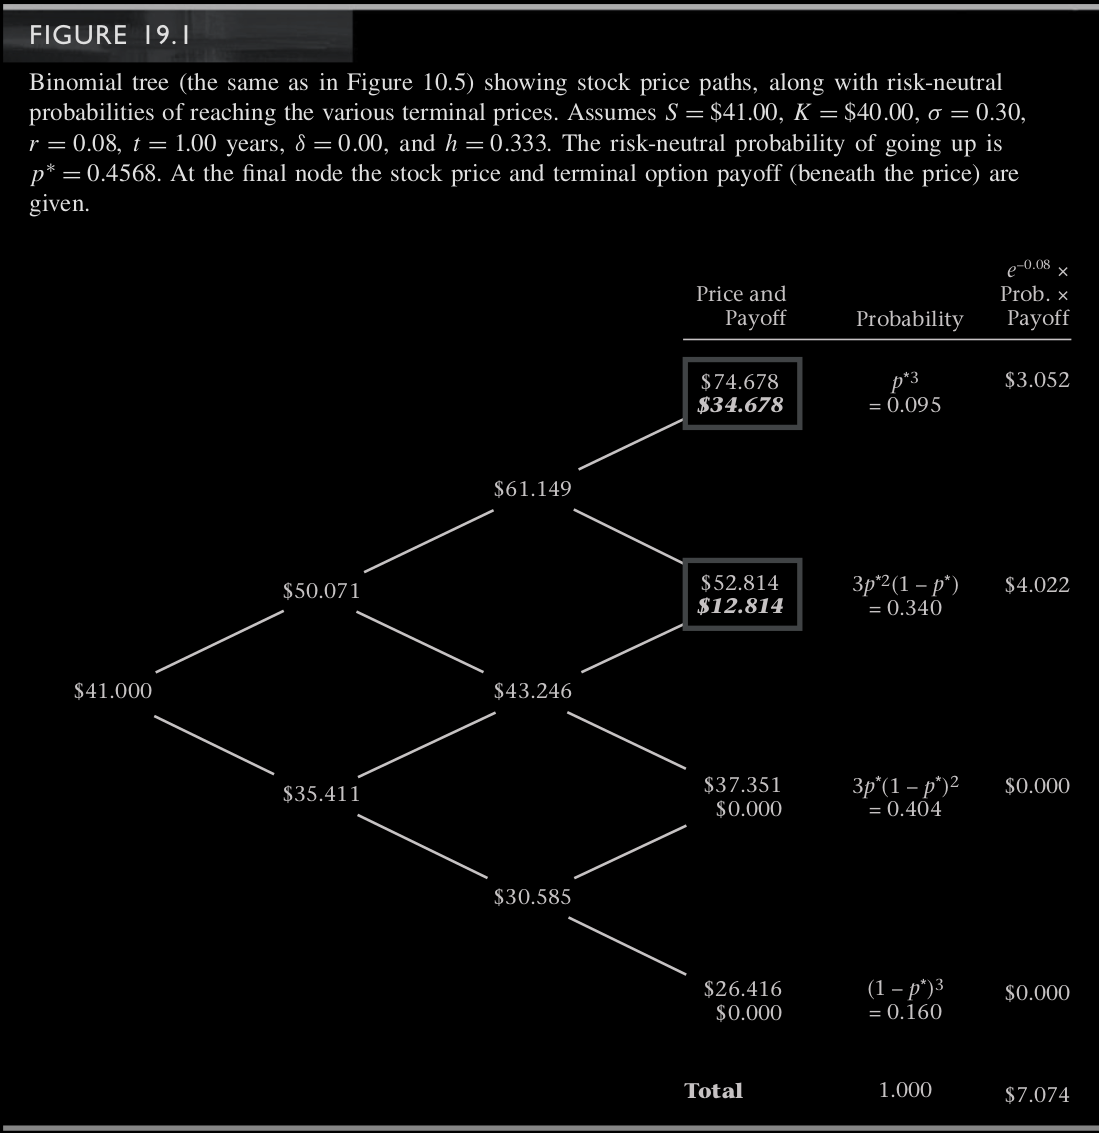
\includegraphics[scale=0.25]{figs/Figure_19-1.png}
\end{center}
\end{frame}
%-------------- end slide -------------------------------%}}}
%-------------- start slide -------------------------------%{{{ 1
\begin{frame}[fragile,t]
Instead of using the formula to compute the option price, one can simulate ...
\bigskip

\begin{myexample}
	Write a piece of code to simulate the binomial tree and compute the corresponding average payoff.
\end{myexample}
\bigskip
\begin{mysol}
	Check \\
	\begin{center}
		\textcolor{gray}{codes/Section\_19-1.py}
	\end{center}
	\myEnd
\end{mysol}
\end{frame}
%-------------- end slide -------------------------------%}}}
